
%(BEGIN_QUESTION)
% Copyright 2006, Tony R. Kuphaldt, released under the Creative Commons Attribution License (v 1.0)
% This means you may do almost anything with this work of mine, so long as you give me proper credit

Identify the respective flow characteristic ({\it linear}, {\it equal percentage}, or {\it quick opening}) for each globe valve shown here:

$$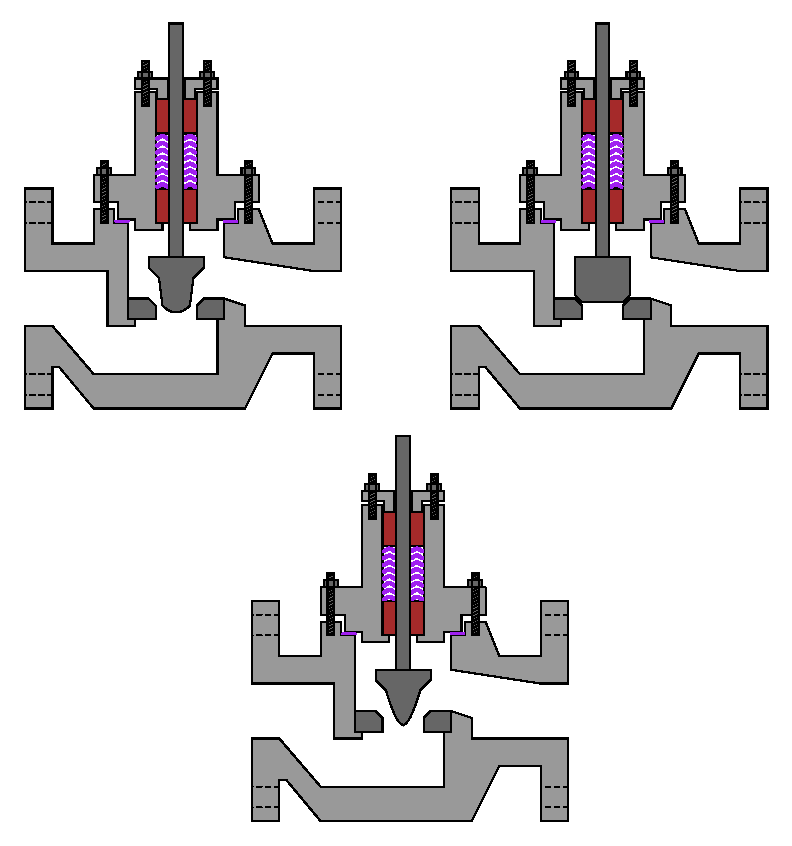
\includegraphics[width=15.5cm]{i01382x01.eps}$$

\vfil \eject

Next, identify the respective flow characteristic ({\it linear}, {\it equal percentage}, or {\it quick opening}) for each rotary ball valve shown here:

$$\includegraphics[width=15.5cm]{i01382x04.eps}$$

\vskip 20pt \vbox{\hrule \hbox{\strut \vrule{} {\bf Suggestions for Socratic discussion} \vrule} \hrule}

\begin{itemize}
\item{} The most important aspect of your answer to this question, as usual, is {\it how} and {\it why} you arrived at your selections.  Explain how you know are able to tell each of these valves' characteristics just from the appearance of the trim cross-sections.
\end{itemize}

\underbar{file i01382}
%(END_QUESTION)





%(BEGIN_ANSWER)

%(END_ANSWER)





%(BEGIN_NOTES)

Identifying linear, equal percentage, and quick opening trim shapes is relatively simple if you have the three different trims side-by-side for comparison.  I like to call this the ``Goldilocks'' method: identifying which is which by comparing their relative shapes one to another.  Linear will be the trim shape that is ``in between'' the two extremes of equal percentage and quick opening.

$$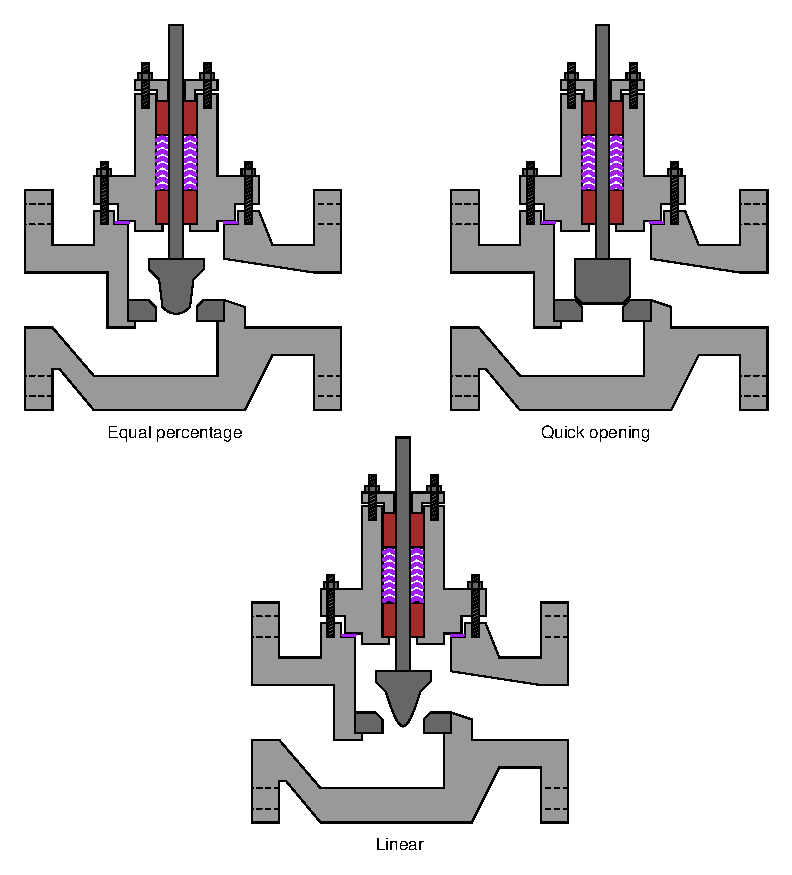
\includegraphics[width=15.5cm]{i01382x02.eps}$$
 
The {\it quick opening} valve should be obvious: it opens up rapidly as the plug moves up off the seat, since the plug does not actually penetrate the ``throat'' of the seat at all, unlike the other trim types.

\vskip 10pt

The bottom valve is {\it linear}, having a nearly perfect cone-shaped plug penetrating through the throat of the seat.  This produces a $C_v$ that varies linearly with plug travel.

\vskip 10pt

The {\it equal percentage} valve is in the upper-left.  Its plug has a much steeper (more vertical) pitch than the linear plug, making its $C_v$ increase at a slower rate at first, but then the plug becomes flatter toward the bottom, making the $C_v$ increase at a more rapid rate toward the end of plug travel.

\vskip 10pt

\filbreak

$$\includegraphics[width=15.5cm]{i01382x05.eps}$$













\vfil \eject

\noindent
{\bf Summary Quiz:}

Select the {\it quick-opening} characteristic globe valve trim:

$$\includegraphics[width=15.5cm]{i01382x03.eps}$$














\vfil \eject

\noindent
{\bf Summary Quiz:}

Select the {\it equal percentage} characteristic globe valve trim:

$$\includegraphics[width=15.5cm]{i01382x03.eps}$$













\vfil \eject

\noindent
{\bf Summary Quiz:}

Select the {\it linear} characteristic globe valve trim:

$$\includegraphics[width=15.5cm]{i01382x03.eps}$$


%INDEX% Final Control Elements, valve: characterization

%(END_NOTES)


